\section{Conclusion}
\label{sec:conclusion}

Summing up, this laboratory provided us the opportunity to understand how the envelope detector and voltage regulator circuits work and, also, how to improve their efficieny.\par
Contrarily to the previous lab assignments, there are some differences between the theoretical and simulation values obtained. This can be explained by the non linear components used in this laboratory: the diodes. In the previous lab assignments only linear components were used and because of that the simple theoretical analysis made matched perfectly the simulation analysis, as it should. This was no longer the case in this assignment. \par
As for the merit figure calculation, we used Spice's values as they provide the most accurate results. \par
Finally, we are going to compare the results from simulation and theoretical analysis side by side: \par
%compararações

\begin{center}
  \begin{tabular}{ | c | c | }
    \hline    
    {\bf Name} & {\bf Value} \\ \hline
    \section{Conclusion}
\label{sec:conclusion}

Summing up, in this laboratory assignment (T2) we have made both theoretical analysis as well as simulations of several different but similar and correlated circuits. \par
The results obtained in both analysis were either put in a table or plotted in order to make comparations between the theoretical and simulation analysis.
The reasoning behind these results is that we studied a very simple circuit containing only linear components. If the components used were more complex, the case would not be the same and we could detect real differences between the values calculated and simulated. \par
That being said we would like to end this report by presenting both the theoretical and simulation results side by side in order to easily compare the results.


\begin{figure}[H]
    \minipage{0.50\textwidth}
      \centering
      \begin{tabular}{ | c | c | }
      \hline    
      {\bf Name} & {\bf Value [A or V]} \\ \hline
      $V_1$ & 5.025226e+00 \\ \hline 
$V_2$ & 4.724476e+00 \\ \hline 
$V_3$ & 4.104661e+00 \\ \hline 
$V_5$ & 4.765766e+00 \\ \hline 
$V_6$ & 5.702373e+00 \\ \hline 
$V_7$ & -1.847813e+00 \\ \hline 
$V_8$ & -2.790649e+00 \\ \hline 
$I_1$ & -2.870701e-04 \\ \hline 
$I_2$ & -3.006765e-04 \\ \hline 
$I_3$ & 1.360640e-05 \\ \hline 
$I_4$ & 1.190255e-03 \\ \hline 
$I_5$ & 3.006765e-04 \\ \hline 
$I_6$ & 9.031846e-04 \\ \hline 
$I_7$ & 9.031846e-04 \\ \hline 
$I_s$ & -2.870701e-04 \\ \hline 
$I_d$ & 9.031846e-04 \\ \hline 
$I_b$ & -3.006765e-04 \\ \hline 
$I_c$ & -2.168404e-19 \\ 

      \hline
      \end{tabular}
      \caption{Theoretical Question 1}
    \endminipage\hfill
    \minipage{0.50\textwidth}
      \centering
      \begin{tabular}{ | c | c | }
      \hline    
      {\bf Name} & {\bf Value [A or V]} \\ \hline
      @c0[i] & 0.000000e+00\\ \hline
@g0[i] & -3.00677e-04\\ \hline
@r1[i] & 2.870701e-04\\ \hline
@r2[i] & -3.00677e-04\\ \hline
@r3[i] & -1.36064e-05\\ \hline
@r4[i] & 1.190255e-03\\ \hline
@r5[i] & -3.00677e-04\\ \hline
@r6[i] & 9.031846e-04\\ \hline
@r7[i] & 9.031846e-04\\ \hline
n1 & 5.025226e+00\\ \hline
n2 & 4.724476e+00\\ \hline
n3 & 4.104661e+00\\ \hline
n5 & 4.765766e+00\\ \hline
n6 & 5.702373e+00\\ \hline
n7 & -1.84781e+00\\ \hline
n8 & -2.79065e+00\\ \hline
n9 & -2.79065e+00\\ \hline

      \end{tabular}
      \caption{Simulation Question 1}
    \endminipage\hfill
\end{figure}

\begin{figure}[H]
    \minipage{0.50\textwidth}
      \centering
      \begin{tabular}{ | c | c | }
      \hline    
      {\bf Name} & {\bf Value [A or V]} \\ \hline
      $V_x$ & 8.493021e+00 \\ \hline 
$V_1$ & 0.000000e+00 \\ \hline 
$V_2$ & 0.000000e+00 \\ \hline 
$V_3$ & -0.000000e+00 \\ \hline 
$V_5$ & 0.000000e+00 \\ \hline 
$V_6$ & 8.493021e+00 \\ \hline 
$V_7$ & 0.000000e+00 \\ \hline 
$V_8$ & 0.000000e+00 \\ \hline 
$I_1$ & 0.000000e+00 \\ \hline 
$I_2$ & 0.000000e+00 \\ \hline 
$I_3$ & 0.000000e+00 \\ \hline 
$I_4$ & 0.000000e+00 \\ \hline 
$I_5$ & 2.726493e-03 \\ \hline 
$I_6$ & -0.000000e+00 \\ \hline 
$I_7$ & -0.000000e+00 \\ \hline 
$I_s$ & 0.000000e+00 \\ \hline 
$I_d$ & -0.000000e+00 \\ \hline 
$I_b$ & 0.000000e+00 \\ \hline 
$I_x$ & 2.726493e-03 \\ \hline 
$Req (kOhm)$ & 3.114999e+00 \\ \hline 
$tau (ms)$ & 3.145605e+00 \\ 

      \hline
      \end{tabular}
      \caption{Theoretical Question 2}
    \endminipage\hfill
    \minipage{0.50\textwidth}
      \centering
      \begin{tabular}{ | c | c | }
      \hline    
      {\bf Name} & {\bf Value [A or V]} \\ \hline
      @g0[i] & 0.000000e+00\\ \hline
@r1[i] & 0.000000e+00\\ \hline
@r2[i] & 0.000000e+00\\ \hline
@r3[i] & 0.000000e+00\\ \hline
@r4[i] & 0.000000e+00\\ \hline
@r5[i] & 2.726492e-03\\ \hline
@r6[i] & 0.000000e+00\\ \hline
@r7[i] & 0.000000e+00\\ \hline
n1 & 0.000000e+00\\ \hline
n2 & 0.000000e+00\\ \hline
n3 & 0.000000e+00\\ \hline
n5 & 0.000000e+00\\ \hline
n6 & -8.49302e+00\\ \hline
n7 & 0.000000e+00\\ \hline
n8 & 0.000000e+00\\ \hline
n9 & 0.000000e+00\\ \hline

      \end{tabular}
      \caption{Simulation Question 2}
    \endminipage\hfill
\end{figure}

\begin{figure}[H]
    \minipage{0.45\textwidth}
      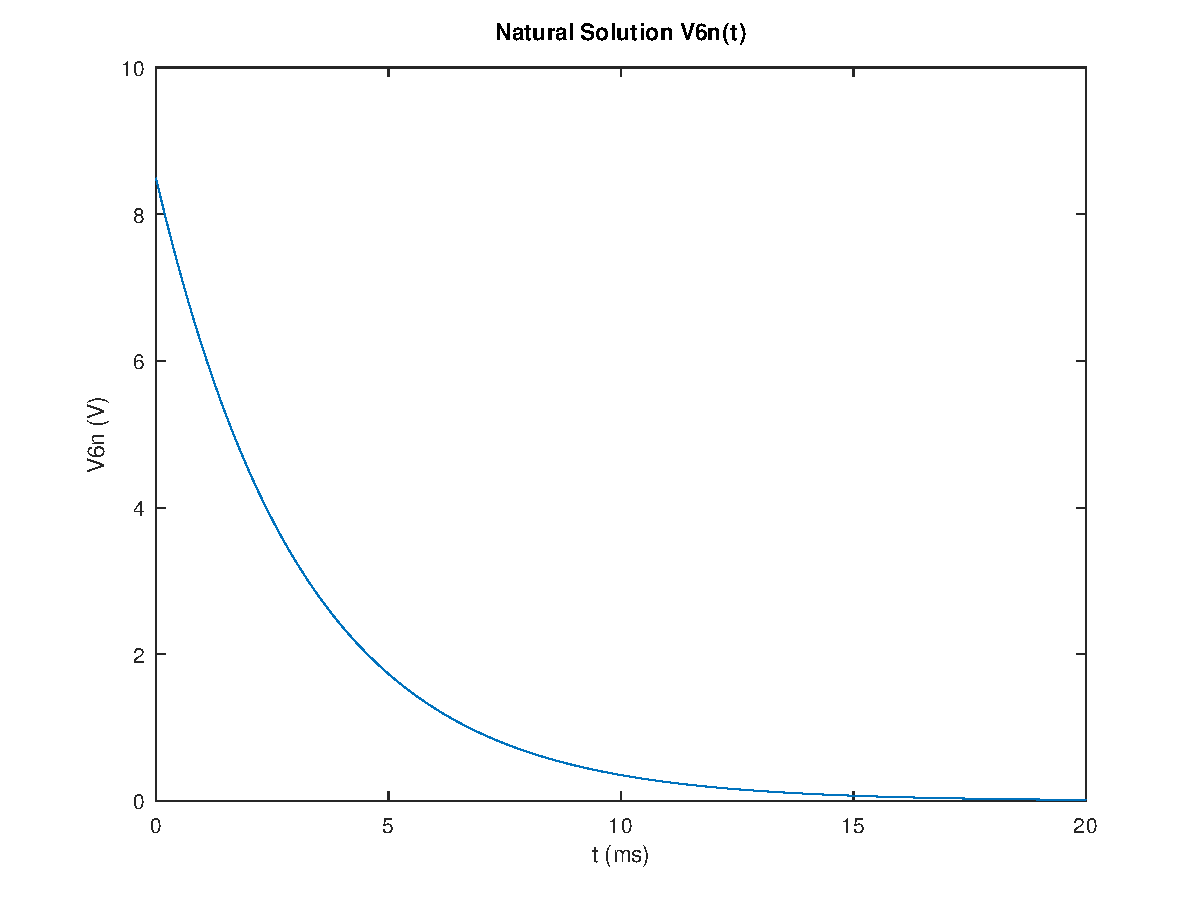
\includegraphics[width=\linewidth]{../mat/alinea3.pdf}
      \caption{Theoretical Question 3}
    \endminipage\hfill
    \minipage{0.45\textwidth}
      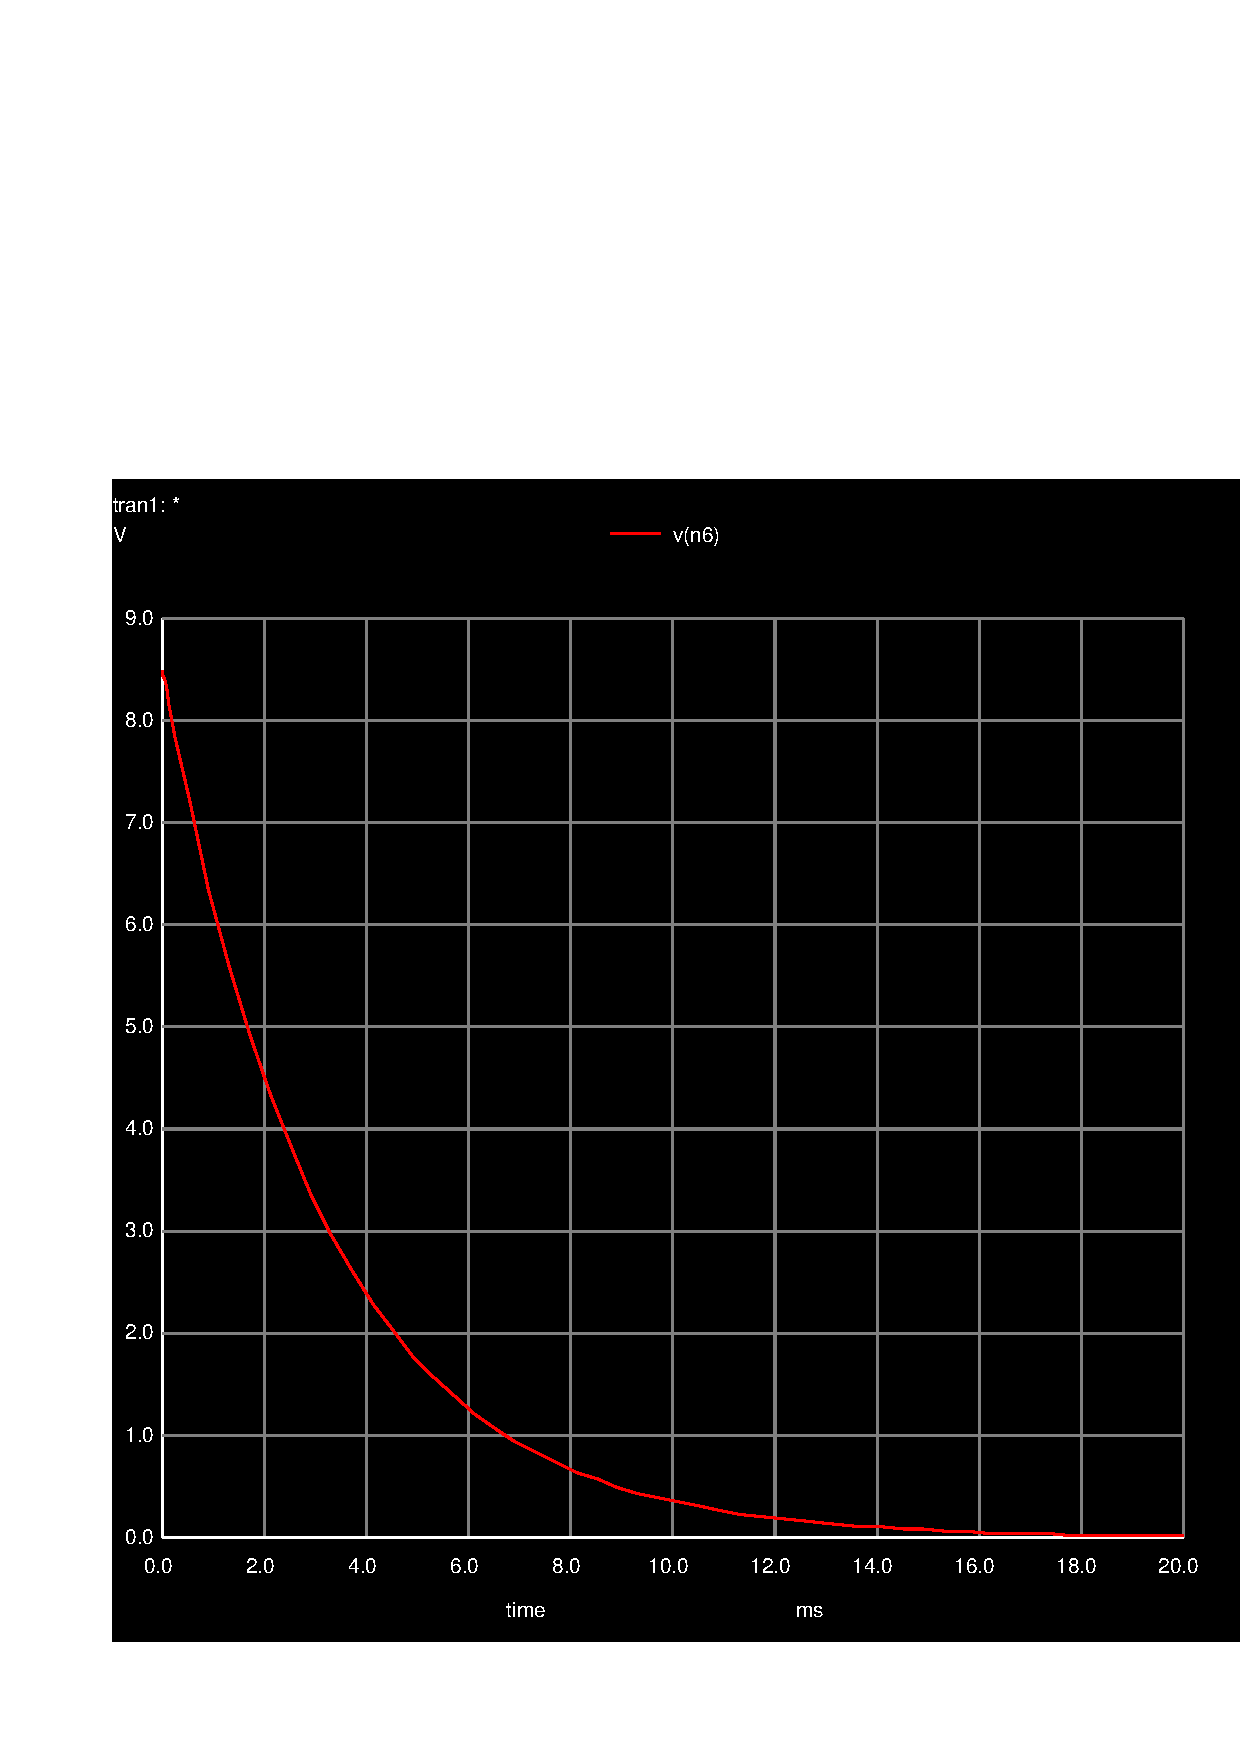
\includegraphics[width=\linewidth]{../sim/transient3.pdf}
      \caption{Simulation Question 3}
    \endminipage\hfill
\end{figure}

\begin{figure}[H]
    \minipage{0.45\textwidth}
      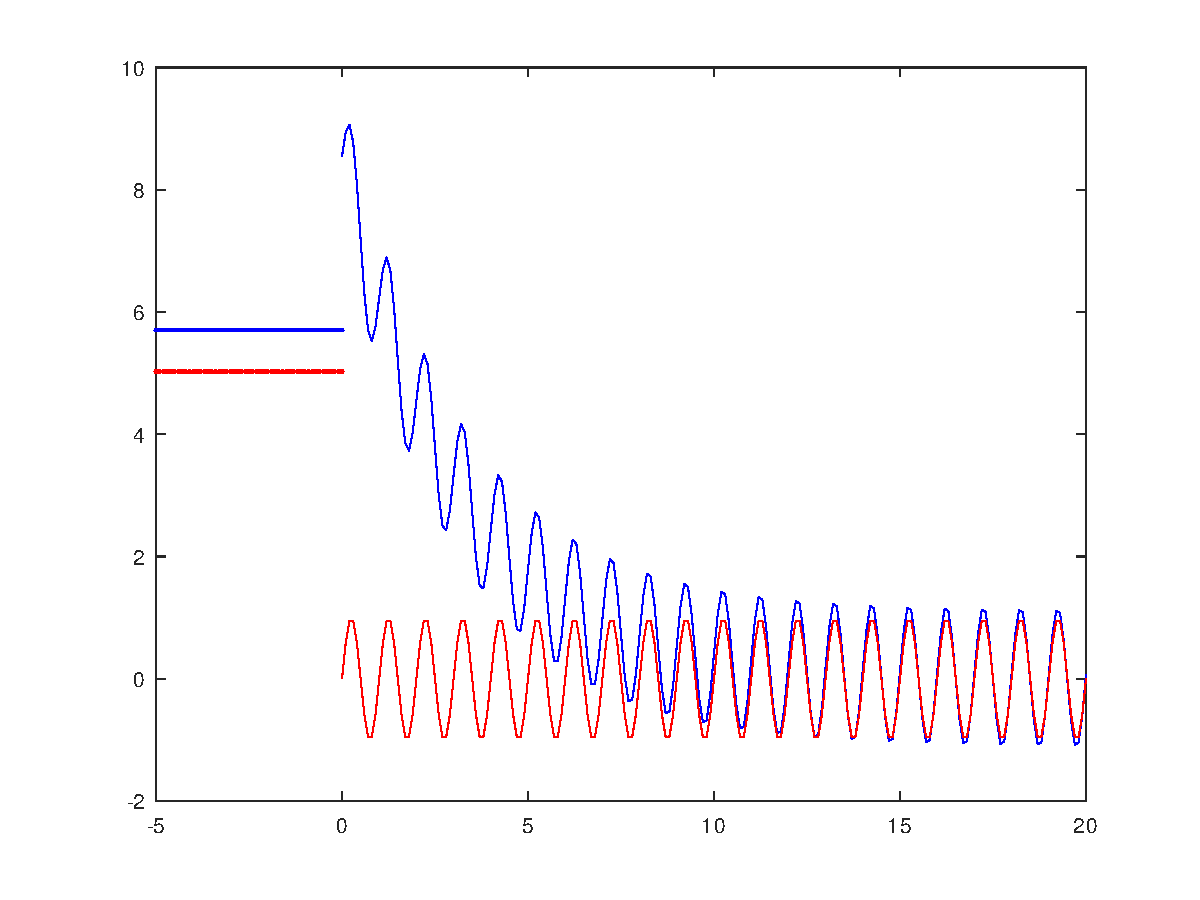
\includegraphics[width=\linewidth]{../mat/alinea5.pdf}
      \caption{Theoretical Question 5}
    \endminipage\hfill
    \minipage{0.45\textwidth}
      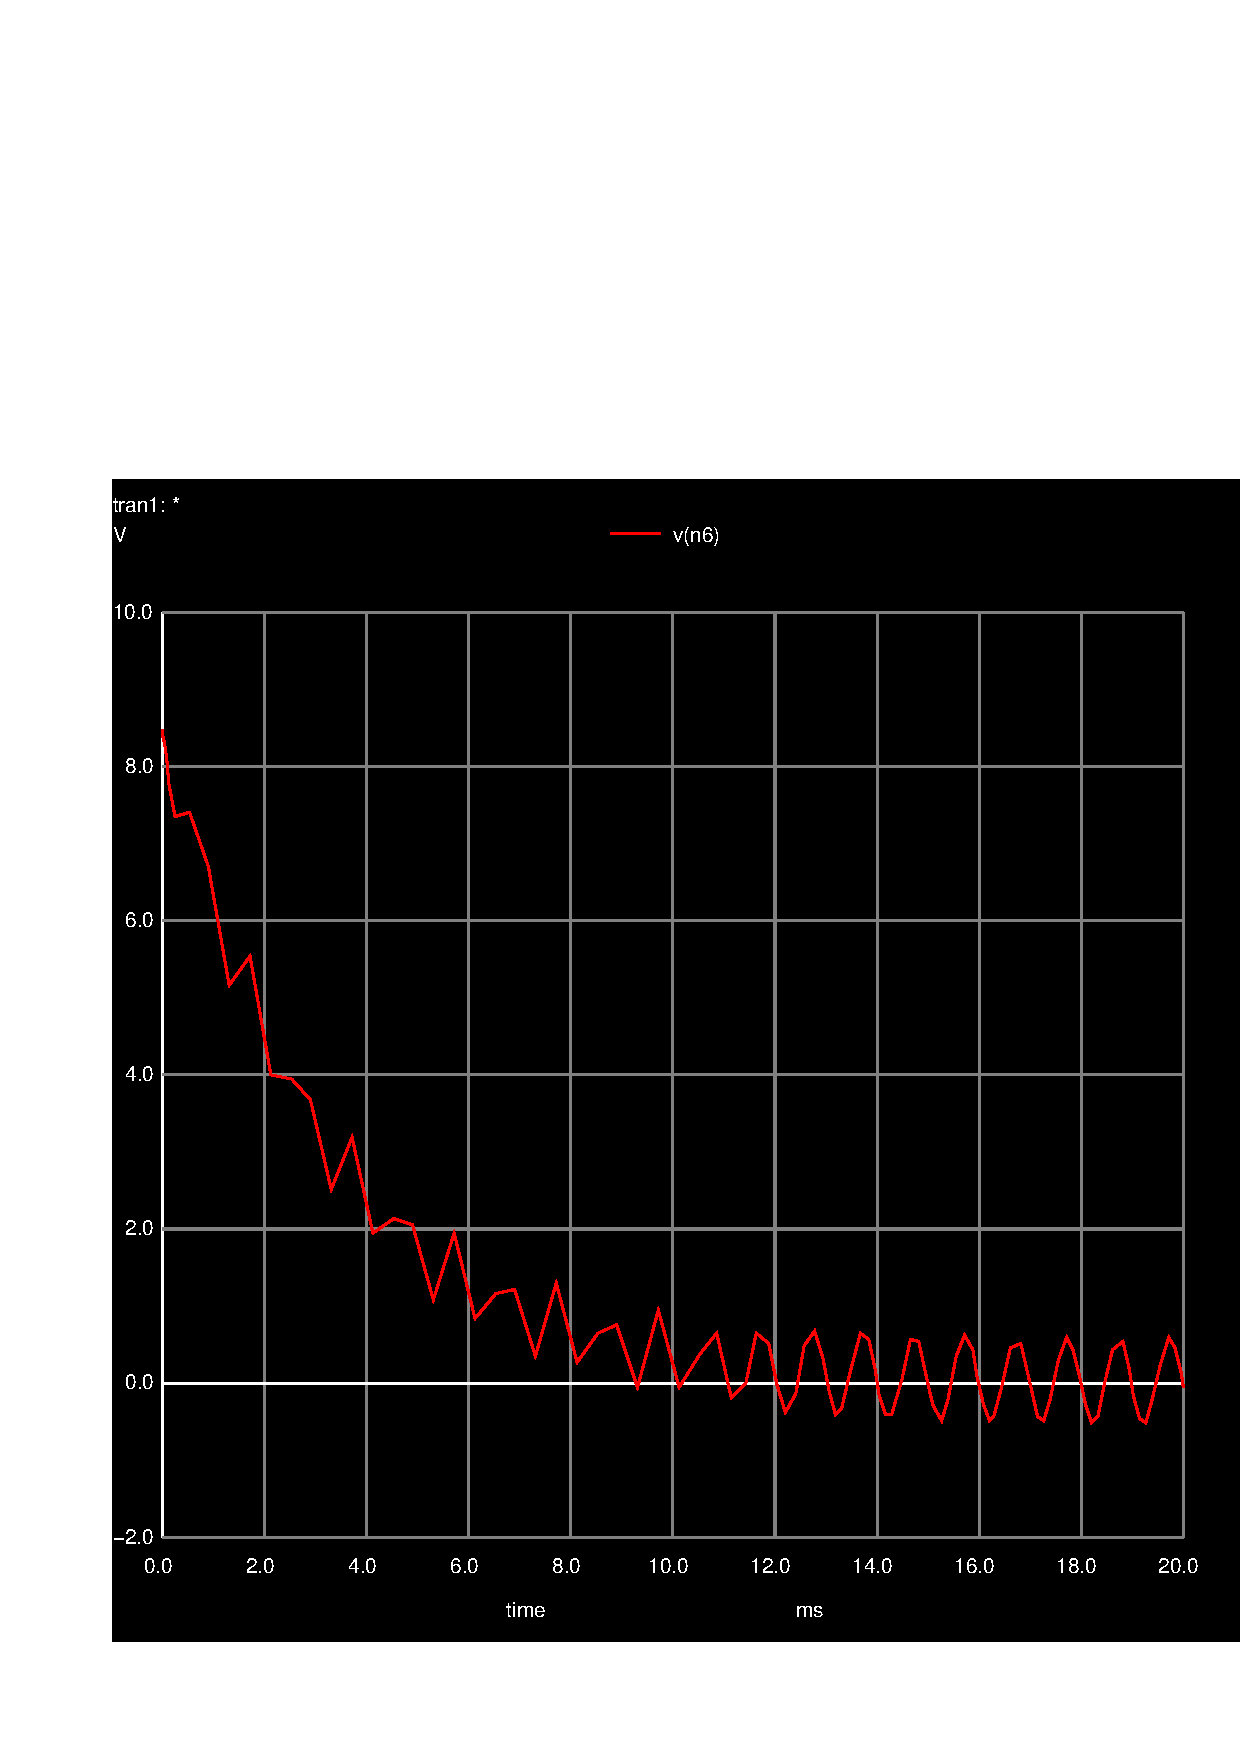
\includegraphics[width=\linewidth]{../sim/transient4r.pdf}
      \caption{Simulation Question 4}
    \endminipage\hfill
\end{figure}

\begin{figure}[H]
    \minipage{0.45\textwidth}
      \includegraphics[width=\linewidth]{../mat/alinea61.pdf}
      \caption{Theoretical Question 6 - Frequency Response}
    \endminipage\hfill
    \minipage{0.45\textwidth}
      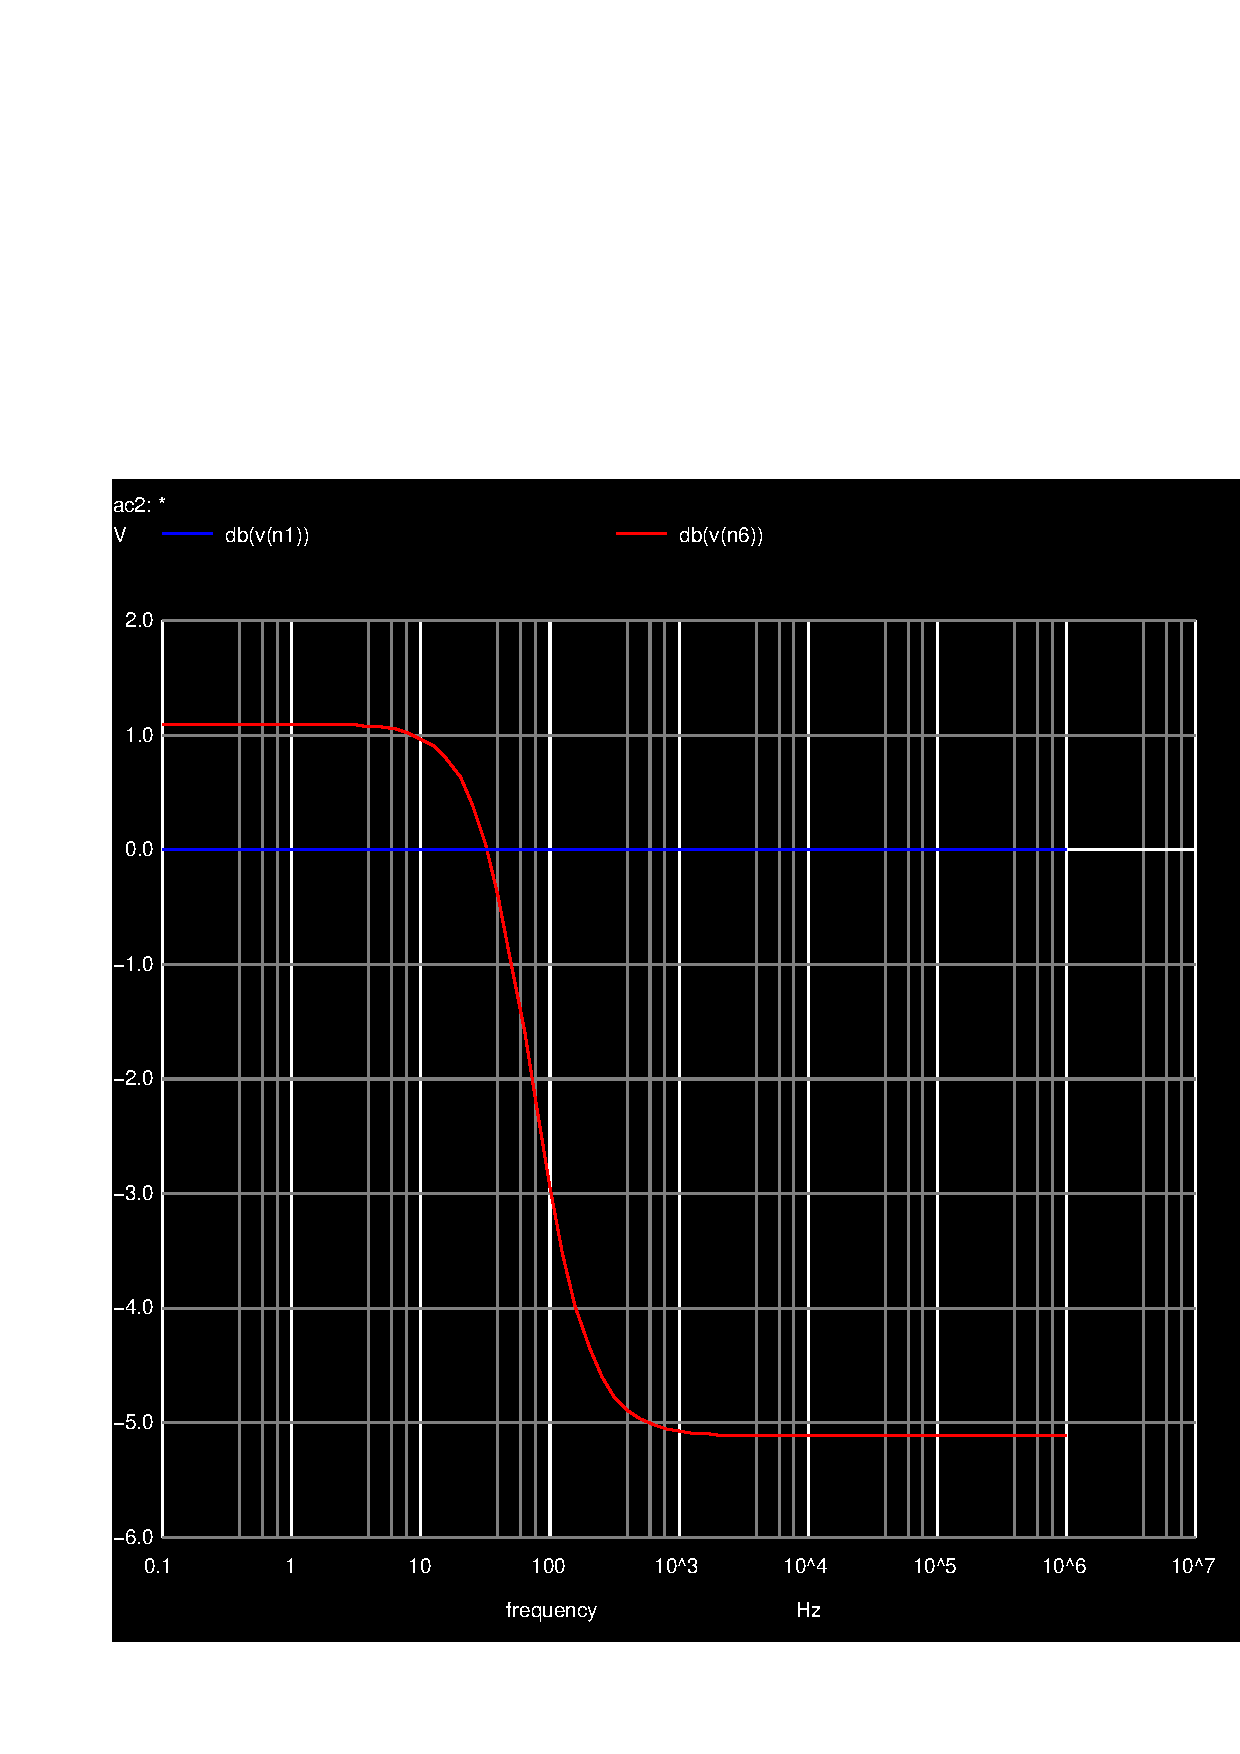
\includegraphics[width=\linewidth]{../sim/fresponse.pdf}
      \caption{Simulation Question 5 - Frequency Response}
    \endminipage\hfill
\end{figure}

    \hline
  \end{tabular}
  \captionof{figure}{Merit Figure Table}
\end{center}

\begin{figure}[H]
    \minipage{0.45\textwidth}
      \includegraphics[width=\linewidth]{../mat/outputdc.pdf}
      \caption{Theoretical Output Voltage Level}
    \endminipage\hfill
    \minipage{0.45\textwidth}
      \includegraphics[width=\linewidth]{../sim/transient1.pdf}
      \caption{Simulation Output Voltage Level}
    \endminipage\hfill
\end{figure}

\begin{center}
  \begin{tabular}{ | c | c | }
    \hline    
    {\bf Name} & {\bf Value [V]} \\ \hline
    \input{../mat/ripple_octave}
  \end{tabular}
  \captionof{figure}{Theoretical Ripple}
\end{center}

\begin{center}
  \begin{tabular}{ | c | c | }
    \hline    
    {\bf Name} & {\bf Value [V]} \\ \hline
    \input{ripple_tab}
  \end{tabular}
  \captionof{figure}{Simulation Ripple}
\end{center}

\begin{figure}[H]
    \minipage{0.45\textwidth}
      \includegraphics[width=\linewidth]{../mat/envelope.pdf}
      \caption{Theoretical Envelope Detector Voltage Level}
    \endminipage\hfill
    \minipage{0.45\textwidth}
      \includegraphics[width=\linewidth]{../sim/transient2.pdf}
      \caption{Simulation Envelope Detector Voltage Level}
    \endminipage\hfill
\end{figure}

\begin{figure}[H]
    \minipage{0.45\textwidth}
      \includegraphics[width=\linewidth]{../mat/outputdc.pdf}
      \caption{Theoretical Voltage Regulator Voltage Level}
    \endminipage\hfill
    \minipage{0.45\textwidth}
      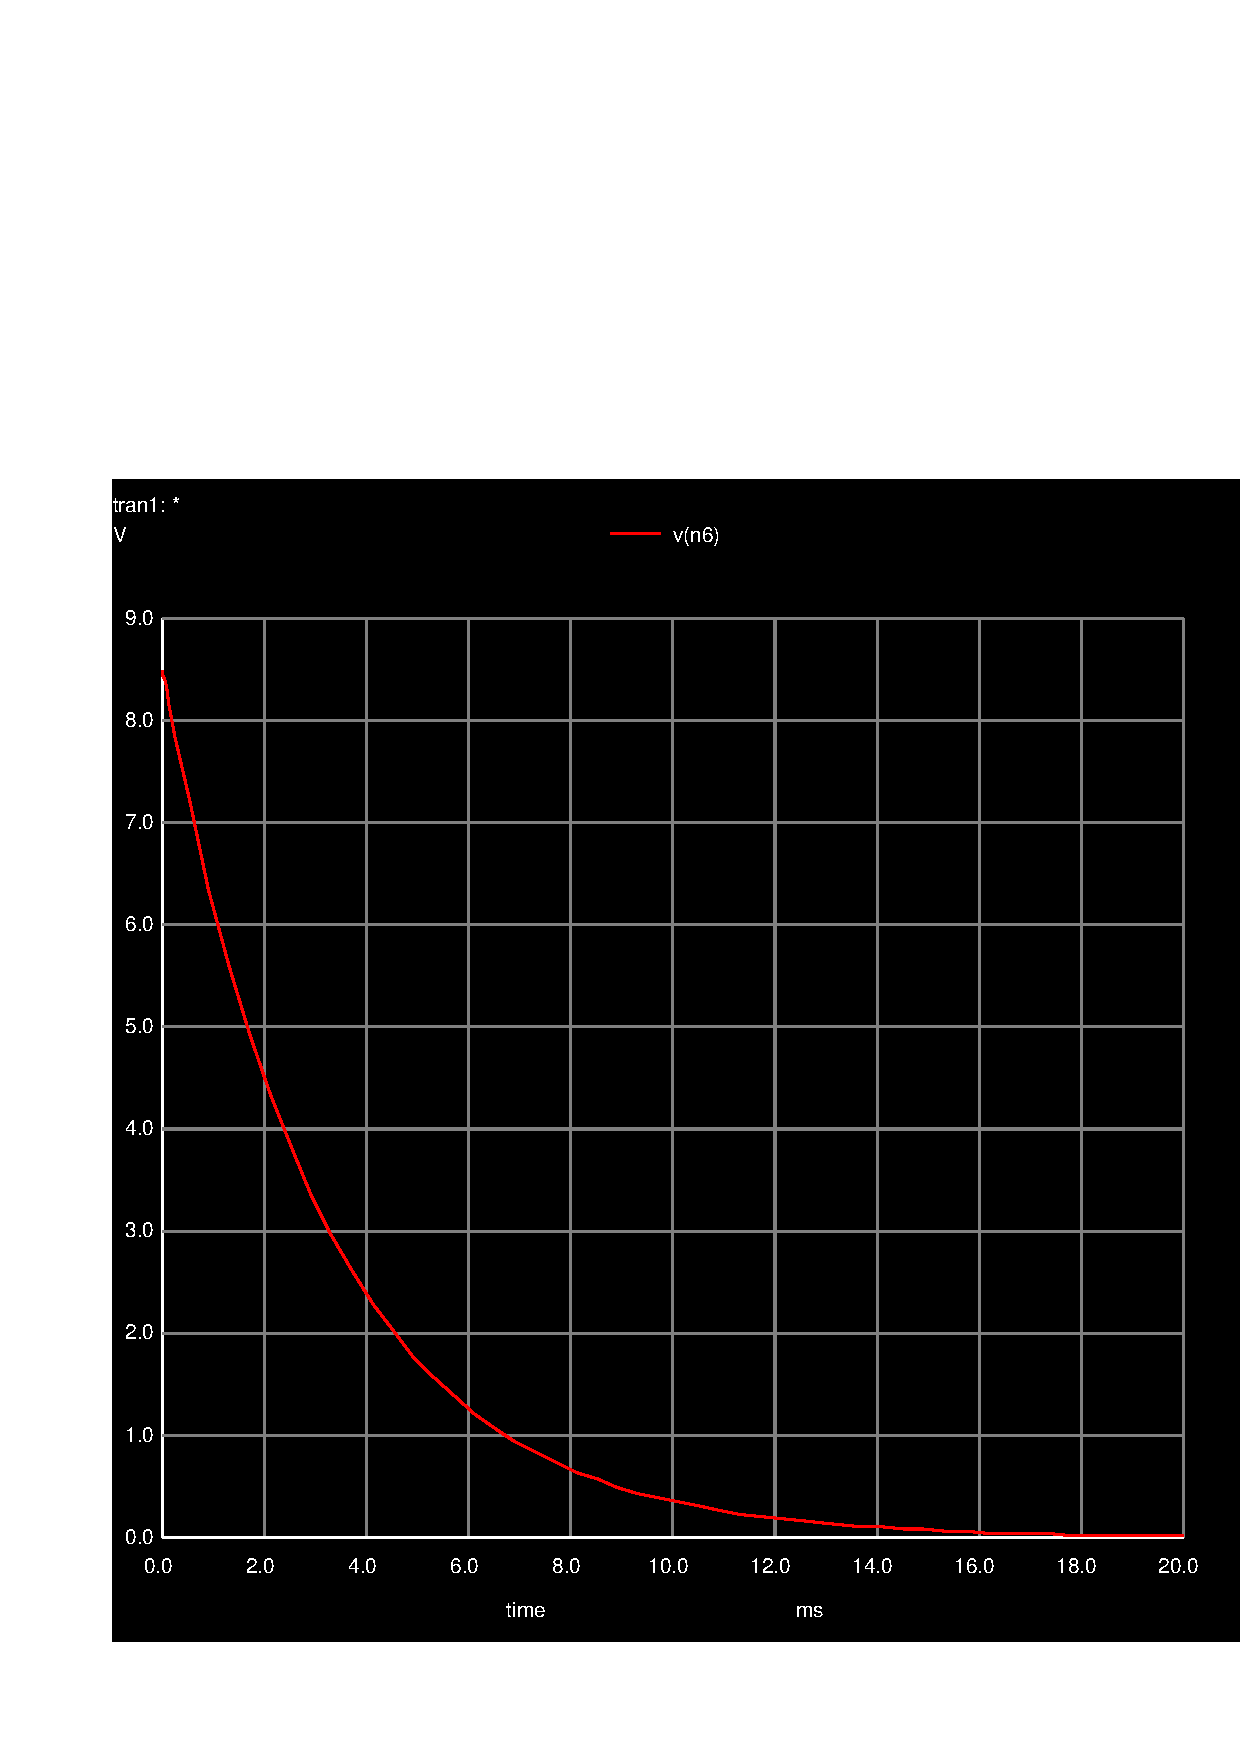
\includegraphics[width=\linewidth]{../sim/transient3.pdf}
      \caption{Simulation Voltage Regulator Voltage Level}
    \endminipage\hfill
\end{figure}

\begin{figure}[H]
    \minipage{0.45\textwidth}
      \includegraphics[width=\linewidth]{../mat/v012.pdf}
      \caption{Theoretical $v_0-12$ Voltage Level}
    \endminipage\hfill
    \minipage{0.45\textwidth}
      \includegraphics[width=\linewidth]{../sim/transient5.pdf}
      \caption{Simulation $v_0-12$ Voltage Level}
    \endminipage\hfill
\end{figure}

